\documentclass[twoside]{book}

% Packages required by doxygen
\usepackage{fixltx2e}
\usepackage{calc}
\usepackage{doxygen}
\usepackage[export]{adjustbox} % also loads graphicx
\usepackage{graphicx}
\usepackage[utf8]{inputenc}
\usepackage{makeidx}
\usepackage{multicol}
\usepackage{multirow}
\PassOptionsToPackage{warn}{textcomp}
\usepackage{textcomp}
\usepackage[nointegrals]{wasysym}
\usepackage[table]{xcolor}

% Font selection
\usepackage[T1]{fontenc}
\usepackage[scaled=.90]{helvet}
\usepackage{courier}
\usepackage{amssymb}
\usepackage{sectsty}
\renewcommand{\familydefault}{\sfdefault}
\allsectionsfont{%
  \fontseries{bc}\selectfont%
  \color{darkgray}%
}
\renewcommand{\DoxyLabelFont}{%
  \fontseries{bc}\selectfont%
  \color{darkgray}%
}
\newcommand{\+}{\discretionary{\mbox{\scriptsize$\hookleftarrow$}}{}{}}

% Page & text layout
\usepackage{geometry}
\geometry{%
  a4paper,%
  top=2.5cm,%
  bottom=2.5cm,%
  left=2.5cm,%
  right=2.5cm%
}
\tolerance=750
\hfuzz=15pt
\hbadness=750
\setlength{\emergencystretch}{15pt}
\setlength{\parindent}{0cm}
\setlength{\parskip}{3ex plus 2ex minus 2ex}
\makeatletter
\renewcommand{\paragraph}{%
  \@startsection{paragraph}{4}{0ex}{-1.0ex}{1.0ex}{%
    \normalfont\normalsize\bfseries\SS@parafont%
  }%
}
\renewcommand{\subparagraph}{%
  \@startsection{subparagraph}{5}{0ex}{-1.0ex}{1.0ex}{%
    \normalfont\normalsize\bfseries\SS@subparafont%
  }%
}
\makeatother

% Headers & footers
\usepackage{fancyhdr}
\pagestyle{fancyplain}
\fancyhead[LE]{\fancyplain{}{\bfseries\thepage}}
\fancyhead[CE]{\fancyplain{}{}}
\fancyhead[RE]{\fancyplain{}{\bfseries\leftmark}}
\fancyhead[LO]{\fancyplain{}{\bfseries\rightmark}}
\fancyhead[CO]{\fancyplain{}{}}
\fancyhead[RO]{\fancyplain{}{\bfseries\thepage}}
\fancyfoot[LE]{\fancyplain{}{}}
\fancyfoot[CE]{\fancyplain{}{}}
\fancyfoot[RE]{\fancyplain{}{\bfseries\scriptsize Generated by Doxygen }}
\fancyfoot[LO]{\fancyplain{}{\bfseries\scriptsize Generated by Doxygen }}
\fancyfoot[CO]{\fancyplain{}{}}
\fancyfoot[RO]{\fancyplain{}{}}
\renewcommand{\footrulewidth}{0.4pt}
\renewcommand{\chaptermark}[1]{%
  \markboth{#1}{}%
}
\renewcommand{\sectionmark}[1]{%
  \markright{\thesection\ #1}%
}

% Indices & bibliography
\usepackage{natbib}
\usepackage[titles]{tocloft}
\setcounter{tocdepth}{3}
\setcounter{secnumdepth}{5}
\makeindex

% Hyperlinks (required, but should be loaded last)
\usepackage{ifpdf}
\ifpdf
  \usepackage[pdftex,pagebackref=true]{hyperref}
\else
  \usepackage[ps2pdf,pagebackref=true]{hyperref}
\fi
\hypersetup{%
  colorlinks=true,%
  linkcolor=blue,%
  citecolor=blue,%
  unicode%
}

% Custom commands
\newcommand{\clearemptydoublepage}{%
  \newpage{\pagestyle{empty}\cleardoublepage}%
}

\usepackage{caption}
\captionsetup{labelsep=space,justification=centering,font={bf},singlelinecheck=off,skip=4pt,position=top}

%===== C O N T E N T S =====

\begin{document}

% Titlepage & ToC
\hypersetup{pageanchor=false,
             bookmarksnumbered=true,
             pdfencoding=unicode
            }
\pagenumbering{roman}
\begin{titlepage}
\vspace*{7cm}
\begin{center}%
{\Large My Project }\\
\vspace*{1cm}
{\large Generated by Doxygen 1.8.11}\\
\end{center}
\end{titlepage}
\clearemptydoublepage
\tableofcontents
\clearemptydoublepage
\pagenumbering{arabic}
\hypersetup{pageanchor=true}

%--- Begin generated contents ---
\chapter{Class Index}
\section{Class List}
Here are the classes, structs, unions and interfaces with brief descriptions\+:\begin{DoxyCompactList}
\item\contentsline{section}{\hyperlink{class__2D__file}{\+\_\+2\+D\+\_\+file} }{\pageref{class__2D__file}}{}
\item\contentsline{section}{\hyperlink{class__3D__file}{\+\_\+3\+D\+\_\+file} }{\pageref{class__3D__file}}{}
\item\contentsline{section}{\hyperlink{structco__ordinates__2D}{co\+\_\+ordinates\+\_\+2D} }{\pageref{structco__ordinates__2D}}{}
\item\contentsline{section}{\hyperlink{structco__ordinates__3D}{co\+\_\+ordinates\+\_\+3D} }{\pageref{structco__ordinates__3D}}{}
\item\contentsline{section}{\hyperlink{classconversion}{conversion} }{\pageref{classconversion}}{}
\item\contentsline{section}{\hyperlink{classfile__3D__temp}{file\+\_\+3\+D\+\_\+temp} }{\pageref{classfile__3D__temp}}{}
\item\contentsline{section}{\hyperlink{classMaster}{Master} }{\pageref{classMaster}}{}
\item\contentsline{section}{\hyperlink{classprojection}{projection} }{\pageref{classprojection}}{}
\item\contentsline{section}{\hyperlink{classtrans}{trans} }{\pageref{classtrans}}{}
\item\contentsline{section}{\hyperlink{structvertex}{vertex} }{\pageref{structvertex}}{}
\end{DoxyCompactList}

\chapter{File Index}
\section{File List}
Here is a list of all files with brief descriptions\+:\begin{DoxyCompactList}
\item\contentsline{section}{include/\hyperlink{2D__file_8h}{2\+D\+\_\+file.\+h} }{\pageref{2D__file_8h}}{}
\item\contentsline{section}{include/\hyperlink{3D__file_8h}{3\+D\+\_\+file.\+h} }{\pageref{3D__file_8h}}{}
\item\contentsline{section}{include/\hyperlink{conversion_8h}{conversion.\+h} }{\pageref{conversion_8h}}{}
\item\contentsline{section}{include/\hyperlink{file__3D__temp_8h}{file\+\_\+3\+D\+\_\+temp.\+h} }{\pageref{file__3D__temp_8h}}{}
\item\contentsline{section}{include/\hyperlink{graph_8h}{graph.\+h} }{\pageref{graph_8h}}{}
\item\contentsline{section}{include/\hyperlink{projection_8h}{projection.\+h} }{\pageref{projection_8h}}{}
\item\contentsline{section}{include/\hyperlink{transform_8h}{transform.\+h} }{\pageref{transform_8h}}{}
\item\contentsline{section}{src/\hyperlink{2D__file_8cpp}{2\+D\+\_\+file.\+cpp} }{\pageref{2D__file_8cpp}}{}
\item\contentsline{section}{src/\hyperlink{3D__file_8cpp}{3\+D\+\_\+file.\+cpp} }{\pageref{3D__file_8cpp}}{}
\item\contentsline{section}{src/\hyperlink{conversion_8cpp}{conversion.\+cpp} }{\pageref{conversion_8cpp}}{}
\item\contentsline{section}{src/\hyperlink{file__3D__temp_8cpp}{file\+\_\+3\+D\+\_\+temp.\+cpp} }{\pageref{file__3D__temp_8cpp}}{}
\item\contentsline{section}{src/\hyperlink{main_8cpp}{main.\+cpp} }{\pageref{main_8cpp}}{}
\item\contentsline{section}{src/\hyperlink{projection_8cpp}{projection.\+cpp} }{\pageref{projection_8cpp}}{}
\item\contentsline{section}{src/\hyperlink{transform_8cpp}{transform.\+cpp} }{\pageref{transform_8cpp}}{}
\end{DoxyCompactList}

\chapter{Class Documentation}
\hypertarget{class__2D__file}{}\section{\+\_\+2\+D\+\_\+file Class Reference}
\label{class__2D__file}\index{\+\_\+2\+D\+\_\+file@{\+\_\+2\+D\+\_\+file}}


Collaboration diagram for \+\_\+2\+D\+\_\+file\+:
\nopagebreak
\begin{figure}[H]
\begin{center}
\leavevmode
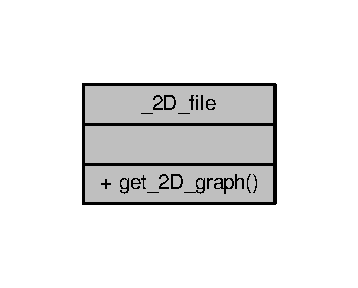
\includegraphics[width=172pt]{class__2D__file__coll__graph}
\end{center}
\end{figure}
\subsection*{Public Member Functions}
\begin{DoxyCompactItemize}
\item 
string \hyperlink{class__2D__file_a7486d81910550512d489c42e02d853b3}{get\+\_\+2\+D\+\_\+graph} (vector$<$ vector$<$ \hyperlink{structco__ordinates__2D}{co\+\_\+ordinates\+\_\+2D} $>$ $>$ \&cz, vector$<$ string $>$ \&edges1, vector$<$ string $>$ \&edges2, vector$<$ string $>$ \&edges3)
\end{DoxyCompactItemize}


\subsection{Member Function Documentation}
\index{\+\_\+2\+D\+\_\+file@{\+\_\+2\+D\+\_\+file}!get\+\_\+2\+D\+\_\+graph@{get\+\_\+2\+D\+\_\+graph}}
\index{get\+\_\+2\+D\+\_\+graph@{get\+\_\+2\+D\+\_\+graph}!\+\_\+2\+D\+\_\+file@{\+\_\+2\+D\+\_\+file}}
\subsubsection[{\texorpdfstring{get\+\_\+2\+D\+\_\+graph(vector$<$ vector$<$ co\+\_\+ordinates\+\_\+2\+D $>$ $>$ \&cz, vector$<$ string $>$ \&edges1, vector$<$ string $>$ \&edges2, vector$<$ string $>$ \&edges3)}{get_2D_graph(vector< vector< co_ordinates_2D > > &cz, vector< string > &edges1, vector< string > &edges2, vector< string > &edges3)}}]{\setlength{\rightskip}{0pt plus 5cm}string \+\_\+2\+D\+\_\+file\+::get\+\_\+2\+D\+\_\+graph (
\begin{DoxyParamCaption}
\item[{vector$<$ vector$<$ {\bf co\+\_\+ordinates\+\_\+2D} $>$ $>$ \&}]{cz, }
\item[{vector$<$ string $>$ \&}]{edges1, }
\item[{vector$<$ string $>$ \&}]{edges2, }
\item[{vector$<$ string $>$ \&}]{edges3}
\end{DoxyParamCaption}
)\hspace{0.3cm}{\ttfamily [inline]}}\hypertarget{class__2D__file_a7486d81910550512d489c42e02d853b3}{}\label{class__2D__file_a7486d81910550512d489c42e02d853b3}
This function prompts the user to first enter the name of the input file containing the vertices(along with co-\/ordinates) and edges of the 3 views of 3\+D-\/figure to be generated. It stores the 2\+D-\/figures in a graph (outgraphs2) and the edges of the 3 views separately. 

The documentation for this class was generated from the following file\+:\begin{DoxyCompactItemize}
\item 
src/\hyperlink{2D__file_8cpp}{2\+D\+\_\+file.\+cpp}\end{DoxyCompactItemize}

\hypertarget{class__3D__file}{}\section{\+\_\+3\+D\+\_\+file Class Reference}
\label{class__3D__file}\index{\+\_\+3\+D\+\_\+file@{\+\_\+3\+D\+\_\+file}}


Collaboration diagram for \+\_\+3\+D\+\_\+file\+:
\nopagebreak
\begin{figure}[H]
\begin{center}
\leavevmode
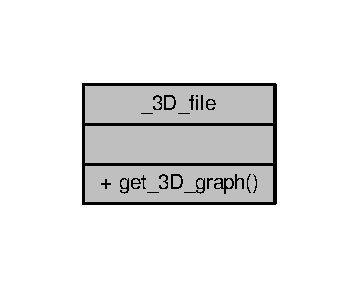
\includegraphics[width=172pt]{class__3D__file__coll__graph}
\end{center}
\end{figure}
\subsection*{Public Member Functions}
\begin{DoxyCompactItemize}
\item 
string \hyperlink{class__3D__file_a7ccd75a68f51eeadb58b3666930160df}{get\+\_\+3\+D\+\_\+graph} (vector$<$ \hyperlink{structco__ordinates__3D}{co\+\_\+ordinates\+\_\+3D} $>$ \&c, vector$<$ string $>$ \&faces)
\end{DoxyCompactItemize}


\subsection{Member Function Documentation}
\index{\+\_\+3\+D\+\_\+file@{\+\_\+3\+D\+\_\+file}!get\+\_\+3\+D\+\_\+graph@{get\+\_\+3\+D\+\_\+graph}}
\index{get\+\_\+3\+D\+\_\+graph@{get\+\_\+3\+D\+\_\+graph}!\+\_\+3\+D\+\_\+file@{\+\_\+3\+D\+\_\+file}}
\subsubsection[{\texorpdfstring{get\+\_\+3\+D\+\_\+graph(vector$<$ co\+\_\+ordinates\+\_\+3\+D $>$ \&c, vector$<$ string $>$ \&faces)}{get_3D_graph(vector< co_ordinates_3D > &c, vector< string > &faces)}}]{\setlength{\rightskip}{0pt plus 5cm}string \+\_\+3\+D\+\_\+file\+::get\+\_\+3\+D\+\_\+graph (
\begin{DoxyParamCaption}
\item[{vector$<$ {\bf co\+\_\+ordinates\+\_\+3D} $>$ \&}]{c, }
\item[{vector$<$ string $>$ \&}]{faces}
\end{DoxyParamCaption}
)\hspace{0.3cm}{\ttfamily [inline]}}\hypertarget{class__3D__file_a7ccd75a68f51eeadb58b3666930160df}{}\label{class__3D__file_a7ccd75a68f51eeadb58b3666930160df}
Firstly, the user is prompted to input a file containing the 3\+D-\/figure and it is stored in a graph. As we are generating 3D view along with the orthographic views, we applied certain transformations, i.\+e. rotation, translation and scaling to get a renderable isometric view. Then the faces which will be visible from the isometric view are generated and stored in a vector(faces). The renderable isometric view generated is stored in a file so that the main function can render it. 

The documentation for this class was generated from the following file\+:\begin{DoxyCompactItemize}
\item 
src/\hyperlink{3D__file_8cpp}{3\+D\+\_\+file.\+cpp}\end{DoxyCompactItemize}

\hypertarget{structco__ordinates__2D}{}\section{co\+\_\+ordinates\+\_\+2D Struct Reference}
\label{structco__ordinates__2D}\index{co\+\_\+ordinates\+\_\+2D@{co\+\_\+ordinates\+\_\+2D}}


{\ttfamily \#include $<$graph.\+h$>$}



Collaboration diagram for co\+\_\+ordinates\+\_\+2D\+:
\nopagebreak
\begin{figure}[H]
\begin{center}
\leavevmode
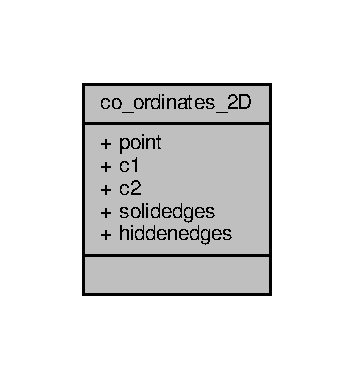
\includegraphics[width=170pt]{structco__ordinates__2D__coll__graph}
\end{center}
\end{figure}
\subsection*{Public Attributes}
\begin{DoxyCompactItemize}
\item 
string \hyperlink{structco__ordinates__2D_a670541bafcbb4094ed3423f655a66cf6}{point}
\item 
float \hyperlink{structco__ordinates__2D_a215c40478ad8333a7c0ab634a6bad587}{c1}
\item 
float \hyperlink{structco__ordinates__2D_ab2320185357bf9635b33b98edb8087f1}{c2}
\item 
vector$<$ string $>$ \hyperlink{structco__ordinates__2D_ab653d4ba438344c0564e74338b58d822}{solidedges}
\item 
vector$<$ string $>$ \hyperlink{structco__ordinates__2D_af5578efed44d03526239551b041aded4}{hiddenedges}
\end{DoxyCompactItemize}


\subsection{Member Data Documentation}
\index{co\+\_\+ordinates\+\_\+2D@{co\+\_\+ordinates\+\_\+2D}!c1@{c1}}
\index{c1@{c1}!co\+\_\+ordinates\+\_\+2D@{co\+\_\+ordinates\+\_\+2D}}
\subsubsection[{\texorpdfstring{c1}{c1}}]{\setlength{\rightskip}{0pt plus 5cm}float co\+\_\+ordinates\+\_\+2\+D\+::c1}\hypertarget{structco__ordinates__2D_a215c40478ad8333a7c0ab634a6bad587}{}\label{structco__ordinates__2D_a215c40478ad8333a7c0ab634a6bad587}
\index{co\+\_\+ordinates\+\_\+2D@{co\+\_\+ordinates\+\_\+2D}!c2@{c2}}
\index{c2@{c2}!co\+\_\+ordinates\+\_\+2D@{co\+\_\+ordinates\+\_\+2D}}
\subsubsection[{\texorpdfstring{c2}{c2}}]{\setlength{\rightskip}{0pt plus 5cm}float co\+\_\+ordinates\+\_\+2\+D\+::c2}\hypertarget{structco__ordinates__2D_ab2320185357bf9635b33b98edb8087f1}{}\label{structco__ordinates__2D_ab2320185357bf9635b33b98edb8087f1}
\index{co\+\_\+ordinates\+\_\+2D@{co\+\_\+ordinates\+\_\+2D}!hiddenedges@{hiddenedges}}
\index{hiddenedges@{hiddenedges}!co\+\_\+ordinates\+\_\+2D@{co\+\_\+ordinates\+\_\+2D}}
\subsubsection[{\texorpdfstring{hiddenedges}{hiddenedges}}]{\setlength{\rightskip}{0pt plus 5cm}vector$<$string$>$ co\+\_\+ordinates\+\_\+2\+D\+::hiddenedges}\hypertarget{structco__ordinates__2D_af5578efed44d03526239551b041aded4}{}\label{structco__ordinates__2D_af5578efed44d03526239551b041aded4}
\index{co\+\_\+ordinates\+\_\+2D@{co\+\_\+ordinates\+\_\+2D}!point@{point}}
\index{point@{point}!co\+\_\+ordinates\+\_\+2D@{co\+\_\+ordinates\+\_\+2D}}
\subsubsection[{\texorpdfstring{point}{point}}]{\setlength{\rightskip}{0pt plus 5cm}string co\+\_\+ordinates\+\_\+2\+D\+::point}\hypertarget{structco__ordinates__2D_a670541bafcbb4094ed3423f655a66cf6}{}\label{structco__ordinates__2D_a670541bafcbb4094ed3423f655a66cf6}
\index{co\+\_\+ordinates\+\_\+2D@{co\+\_\+ordinates\+\_\+2D}!solidedges@{solidedges}}
\index{solidedges@{solidedges}!co\+\_\+ordinates\+\_\+2D@{co\+\_\+ordinates\+\_\+2D}}
\subsubsection[{\texorpdfstring{solidedges}{solidedges}}]{\setlength{\rightskip}{0pt plus 5cm}vector$<$string$>$ co\+\_\+ordinates\+\_\+2\+D\+::solidedges}\hypertarget{structco__ordinates__2D_ab653d4ba438344c0564e74338b58d822}{}\label{structco__ordinates__2D_ab653d4ba438344c0564e74338b58d822}


The documentation for this struct was generated from the following file\+:\begin{DoxyCompactItemize}
\item 
include/\hyperlink{graph_8h}{graph.\+h}\end{DoxyCompactItemize}

\hypertarget{structco__ordinates__3D}{}\section{co\+\_\+ordinates\+\_\+3D Struct Reference}
\label{structco__ordinates__3D}\index{co\+\_\+ordinates\+\_\+3D@{co\+\_\+ordinates\+\_\+3D}}


{\ttfamily \#include $<$graph.\+h$>$}



Collaboration diagram for co\+\_\+ordinates\+\_\+3D\+:
\nopagebreak
\begin{figure}[H]
\begin{center}
\leavevmode
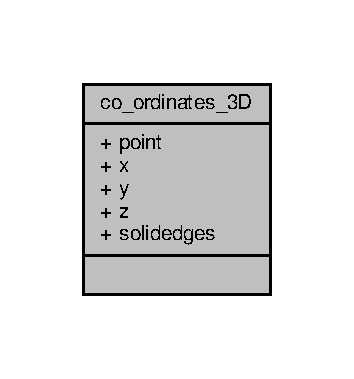
\includegraphics[width=170pt]{structco__ordinates__3D__coll__graph}
\end{center}
\end{figure}
\subsection*{Public Attributes}
\begin{DoxyCompactItemize}
\item 
string \hyperlink{structco__ordinates__3D_a0c51eac3755997b35253e662676391bc}{point}
\item 
float \hyperlink{structco__ordinates__3D_a7fc95a1e0fbe0b7501be1d8e3dcac421}{x}
\item 
float \hyperlink{structco__ordinates__3D_a9d7588247a3b8e2344d213652ec5636a}{y}
\item 
float \hyperlink{structco__ordinates__3D_a900db1bbecab943039799a99ed30428e}{z}
\item 
vector$<$ string $>$ \hyperlink{structco__ordinates__3D_aad059234fd1b769fe491104663a63e77}{solidedges}
\end{DoxyCompactItemize}


\subsection{Member Data Documentation}
\index{co\+\_\+ordinates\+\_\+3D@{co\+\_\+ordinates\+\_\+3D}!point@{point}}
\index{point@{point}!co\+\_\+ordinates\+\_\+3D@{co\+\_\+ordinates\+\_\+3D}}
\subsubsection[{\texorpdfstring{point}{point}}]{\setlength{\rightskip}{0pt plus 5cm}string co\+\_\+ordinates\+\_\+3\+D\+::point}\hypertarget{structco__ordinates__3D_a0c51eac3755997b35253e662676391bc}{}\label{structco__ordinates__3D_a0c51eac3755997b35253e662676391bc}
\index{co\+\_\+ordinates\+\_\+3D@{co\+\_\+ordinates\+\_\+3D}!solidedges@{solidedges}}
\index{solidedges@{solidedges}!co\+\_\+ordinates\+\_\+3D@{co\+\_\+ordinates\+\_\+3D}}
\subsubsection[{\texorpdfstring{solidedges}{solidedges}}]{\setlength{\rightskip}{0pt plus 5cm}vector$<$string$>$ co\+\_\+ordinates\+\_\+3\+D\+::solidedges}\hypertarget{structco__ordinates__3D_aad059234fd1b769fe491104663a63e77}{}\label{structco__ordinates__3D_aad059234fd1b769fe491104663a63e77}
\index{co\+\_\+ordinates\+\_\+3D@{co\+\_\+ordinates\+\_\+3D}!x@{x}}
\index{x@{x}!co\+\_\+ordinates\+\_\+3D@{co\+\_\+ordinates\+\_\+3D}}
\subsubsection[{\texorpdfstring{x}{x}}]{\setlength{\rightskip}{0pt plus 5cm}float co\+\_\+ordinates\+\_\+3\+D\+::x}\hypertarget{structco__ordinates__3D_a7fc95a1e0fbe0b7501be1d8e3dcac421}{}\label{structco__ordinates__3D_a7fc95a1e0fbe0b7501be1d8e3dcac421}
\index{co\+\_\+ordinates\+\_\+3D@{co\+\_\+ordinates\+\_\+3D}!y@{y}}
\index{y@{y}!co\+\_\+ordinates\+\_\+3D@{co\+\_\+ordinates\+\_\+3D}}
\subsubsection[{\texorpdfstring{y}{y}}]{\setlength{\rightskip}{0pt plus 5cm}float co\+\_\+ordinates\+\_\+3\+D\+::y}\hypertarget{structco__ordinates__3D_a9d7588247a3b8e2344d213652ec5636a}{}\label{structco__ordinates__3D_a9d7588247a3b8e2344d213652ec5636a}
\index{co\+\_\+ordinates\+\_\+3D@{co\+\_\+ordinates\+\_\+3D}!z@{z}}
\index{z@{z}!co\+\_\+ordinates\+\_\+3D@{co\+\_\+ordinates\+\_\+3D}}
\subsubsection[{\texorpdfstring{z}{z}}]{\setlength{\rightskip}{0pt plus 5cm}float co\+\_\+ordinates\+\_\+3\+D\+::z}\hypertarget{structco__ordinates__3D_a900db1bbecab943039799a99ed30428e}{}\label{structco__ordinates__3D_a900db1bbecab943039799a99ed30428e}


The documentation for this struct was generated from the following file\+:\begin{DoxyCompactItemize}
\item 
include/\hyperlink{graph_8h}{graph.\+h}\end{DoxyCompactItemize}

\hypertarget{classconversion}{}\section{conversion Class Reference}
\label{classconversion}\index{conversion@{conversion}}


Collaboration diagram for conversion\+:
\nopagebreak
\begin{figure}[H]
\begin{center}
\leavevmode
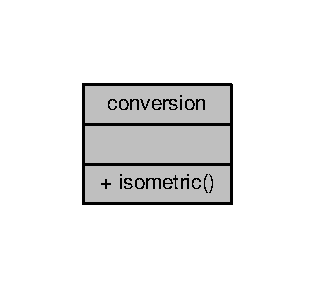
\includegraphics[width=151pt]{classconversion__coll__graph}
\end{center}
\end{figure}
\subsection*{Public Member Functions}
\begin{DoxyCompactItemize}
\item 
void \hyperlink{classconversion_a93f96b765225a746670f804db64416fc}{isometric} (vector$<$ vector$<$ \hyperlink{structco__ordinates__2D}{co\+\_\+ordinates\+\_\+2D} $>$ $>$ outgraphs2, vector$<$ string $>$ edges1, vector$<$ string $>$ edges2, vector$<$ string $>$ edges3)
\end{DoxyCompactItemize}


\subsection{Member Function Documentation}
\index{conversion@{conversion}!isometric@{isometric}}
\index{isometric@{isometric}!conversion@{conversion}}
\subsubsection[{\texorpdfstring{isometric(vector$<$ vector$<$ co\+\_\+ordinates\+\_\+2\+D $>$ $>$ outgraphs2, vector$<$ string $>$ edges1, vector$<$ string $>$ edges2, vector$<$ string $>$ edges3)}{isometric(vector< vector< co_ordinates_2D > > outgraphs2, vector< string > edges1, vector< string > edges2, vector< string > edges3)}}]{\setlength{\rightskip}{0pt plus 5cm}void conversion\+::isometric (
\begin{DoxyParamCaption}
\item[{vector$<$ vector$<$ {\bf co\+\_\+ordinates\+\_\+2D} $>$ $>$}]{outgraphs2, }
\item[{vector$<$ string $>$}]{edges1, }
\item[{vector$<$ string $>$}]{edges2, }
\item[{vector$<$ string $>$}]{edges3}
\end{DoxyParamCaption}
)\hspace{0.3cm}{\ttfamily [inline]}}\hypertarget{classconversion_a93f96b765225a746670f804db64416fc}{}\label{classconversion_a93f96b765225a746670f804db64416fc}
It checks for any inconsistency in the data given ,i.\+e. incompatible views etc in the source graph(outgraphs2). The 3D graph is then generated using point to point correspondence given in the input. After the input given is verified for consistency and the 3\+D-\/graph is generated, the user is given a choice to see the isometric view or view along a general line of sight. If the user wants a general line of sight, he/she has to input the direction vectors of the line of view. After the viewing direction is decided, the co-\/ordinates stored in the graph are rotated and stored in a .txt file in a renderable format for QT and then the control is returned to main function. 

The documentation for this class was generated from the following file\+:\begin{DoxyCompactItemize}
\item 
src/\hyperlink{conversion_8cpp}{conversion.\+cpp}\end{DoxyCompactItemize}

\hypertarget{classfile__3D__temp}{}\section{file\+\_\+3\+D\+\_\+temp Class Reference}
\label{classfile__3D__temp}\index{file\+\_\+3\+D\+\_\+temp@{file\+\_\+3\+D\+\_\+temp}}


Collaboration diagram for file\+\_\+3\+D\+\_\+temp\+:
\nopagebreak
\begin{figure}[H]
\begin{center}
\leavevmode
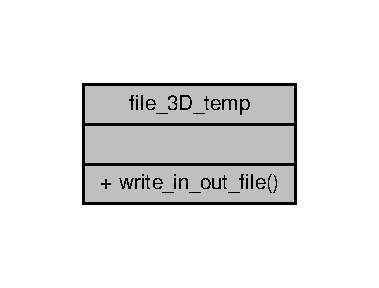
\includegraphics[width=182pt]{classfile__3D__temp__coll__graph}
\end{center}
\end{figure}
\subsection*{Public Member Functions}
\begin{DoxyCompactItemize}
\item 
void \hyperlink{classfile__3D__temp_ab66f68a9494f7bb1db1defc8f31fa233}{write\+\_\+in\+\_\+out\+\_\+file} (vector$<$ vector$<$ \hyperlink{structco__ordinates__2D}{co\+\_\+ordinates\+\_\+2D} $>$ $>$ outgraphs, int choice)
\end{DoxyCompactItemize}


\subsection{Member Function Documentation}
\index{file\+\_\+3\+D\+\_\+temp@{file\+\_\+3\+D\+\_\+temp}!write\+\_\+in\+\_\+out\+\_\+file@{write\+\_\+in\+\_\+out\+\_\+file}}
\index{write\+\_\+in\+\_\+out\+\_\+file@{write\+\_\+in\+\_\+out\+\_\+file}!file\+\_\+3\+D\+\_\+temp@{file\+\_\+3\+D\+\_\+temp}}
\subsubsection[{\texorpdfstring{write\+\_\+in\+\_\+out\+\_\+file(vector$<$ vector$<$ co\+\_\+ordinates\+\_\+2\+D $>$ $>$ outgraphs, int choice)}{write_in_out_file(vector< vector< co_ordinates_2D > > outgraphs, int choice)}}]{\setlength{\rightskip}{0pt plus 5cm}void file\+\_\+3\+D\+\_\+temp\+::write\+\_\+in\+\_\+out\+\_\+file (
\begin{DoxyParamCaption}
\item[{vector$<$ vector$<$ {\bf co\+\_\+ordinates\+\_\+2D} $>$ $>$}]{outgraphs, }
\item[{int}]{choice}
\end{DoxyParamCaption}
)\hspace{0.3cm}{\ttfamily [inline]}}\hypertarget{classfile__3D__temp_ab66f68a9494f7bb1db1defc8f31fa233}{}\label{classfile__3D__temp_ab66f68a9494f7bb1db1defc8f31fa233}
This function prints the 3 2\+D-\/graphs in a .txt file appropriately such that QT can render these graphs easily. It basically stores the graphs in a particular format which can be easily rendered in the main function by QT. 

The documentation for this class was generated from the following file\+:\begin{DoxyCompactItemize}
\item 
src/\hyperlink{file__3D__temp_8cpp}{file\+\_\+3\+D\+\_\+temp.\+cpp}\end{DoxyCompactItemize}

\hypertarget{classMaster}{}\section{Master Class Reference}
\label{classMaster}\index{Master@{Master}}


Collaboration diagram for Master\+:
\nopagebreak
\begin{figure}[H]
\begin{center}
\leavevmode
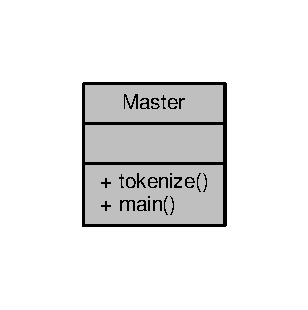
\includegraphics[width=148pt]{classMaster__coll__graph}
\end{center}
\end{figure}
\subsection*{Public Member Functions}
\begin{DoxyCompactItemize}
\item 
void \hyperlink{classMaster_a809ae2b701513e55bef4945be84eb50c}{tokenize} (string a, vector$<$ string $>$ \&vect)
\item 
int \hyperlink{classMaster_ad1ad009b3055a7737ec20aedc788cf6e}{main} ()
\end{DoxyCompactItemize}


\subsection{Detailed Description}
User Mode selection is done here. 

\subsection{Member Function Documentation}
\index{Master@{Master}!main@{main}}
\index{main@{main}!Master@{Master}}
\subsubsection[{\texorpdfstring{main()}{main()}}]{\setlength{\rightskip}{0pt plus 5cm}int Master\+::main (
\begin{DoxyParamCaption}
{}
\end{DoxyParamCaption}
)\hspace{0.3cm}{\ttfamily [inline]}}\hypertarget{classMaster_ad1ad009b3055a7737ec20aedc788cf6e}{}\label{classMaster_ad1ad009b3055a7737ec20aedc788cf6e}
The procedure that has been applied here is \+:
\begin{DoxyEnumerate}
\item Firstly, the user is prompted to input that in which mode he wants to work , 3\+D\+\_\+to\+\_\+2D mode or 2\+D\+\_\+to\+\_\+3D mode.
\item In the second step, the user is directed to functions/methods in other files according to the choice made.
\item When the processing in other files is done, the output file is rendered on a canvas using QT. 
\end{DoxyEnumerate}\index{Master@{Master}!tokenize@{tokenize}}
\index{tokenize@{tokenize}!Master@{Master}}
\subsubsection[{\texorpdfstring{tokenize(string a, vector$<$ string $>$ \&vect)}{tokenize(string a, vector< string > &vect)}}]{\setlength{\rightskip}{0pt plus 5cm}void Master\+::tokenize (
\begin{DoxyParamCaption}
\item[{string}]{a, }
\item[{vector$<$ string $>$ \&}]{vect}
\end{DoxyParamCaption}
)\hspace{0.3cm}{\ttfamily [inline]}}\hypertarget{classMaster_a809ae2b701513e55bef4945be84eb50c}{}\label{classMaster_a809ae2b701513e55bef4945be84eb50c}
This function breaks a string into characters and store them in a vector named vect. 

The documentation for this class was generated from the following file\+:\begin{DoxyCompactItemize}
\item 
src/\hyperlink{main_8cpp}{main.\+cpp}\end{DoxyCompactItemize}

\hypertarget{classprojection}{}\section{projection Class Reference}
\label{classprojection}\index{projection@{projection}}


Collaboration diagram for projection\+:
\nopagebreak
\begin{figure}[H]
\begin{center}
\leavevmode
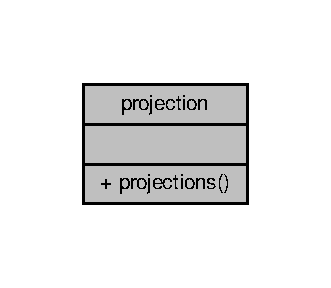
\includegraphics[width=159pt]{classprojection__coll__graph}
\end{center}
\end{figure}
\subsection*{Public Member Functions}
\begin{DoxyCompactItemize}
\item 
void \hyperlink{classprojection_ac3b890ac2ba5979e472742cff14b329a}{projections} (vector$<$ \hyperlink{structco__ordinates__3D}{co\+\_\+ordinates\+\_\+3D} $>$ \&c, vector$<$ vector$<$ \hyperlink{structco__ordinates__2D}{co\+\_\+ordinates\+\_\+2D} $>$ $>$ \&graphs)
\end{DoxyCompactItemize}


\subsection{Member Function Documentation}
\index{projection@{projection}!projections@{projections}}
\index{projections@{projections}!projection@{projection}}
\subsubsection[{\texorpdfstring{projections(vector$<$ co\+\_\+ordinates\+\_\+3\+D $>$ \&c, vector$<$ vector$<$ co\+\_\+ordinates\+\_\+2\+D $>$ $>$ \&graphs)}{projections(vector< co_ordinates_3D > &c, vector< vector< co_ordinates_2D > > &graphs)}}]{\setlength{\rightskip}{0pt plus 5cm}void projection\+::projections (
\begin{DoxyParamCaption}
\item[{vector$<$ {\bf co\+\_\+ordinates\+\_\+3D} $>$ \&}]{c, }
\item[{vector$<$ vector$<$ {\bf co\+\_\+ordinates\+\_\+2D} $>$ $>$ \&}]{graphs}
\end{DoxyParamCaption}
)\hspace{0.3cm}{\ttfamily [inline]}}\hypertarget{classprojection_ac3b890ac2ba5979e472742cff14b329a}{}\label{classprojection_ac3b890ac2ba5979e472742cff14b329a}
In this function the graph containing the transformed 3\+D-\/view is converted into a 3 graphs containing the projections by using various projection matrices for each view and stored in a vector of 2\+D-\/graphs. 

The documentation for this class was generated from the following file\+:\begin{DoxyCompactItemize}
\item 
src/\hyperlink{projection_8cpp}{projection.\+cpp}\end{DoxyCompactItemize}

\hypertarget{classtrans}{}\section{trans Class Reference}
\label{classtrans}\index{trans@{trans}}


Collaboration diagram for trans\+:
\nopagebreak
\begin{figure}[H]
\begin{center}
\leavevmode
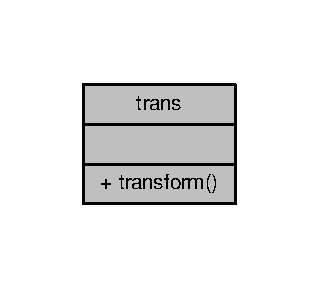
\includegraphics[width=153pt]{classtrans__coll__graph}
\end{center}
\end{figure}
\subsection*{Public Member Functions}
\begin{DoxyCompactItemize}
\item 
int \hyperlink{classtrans_a4b4cf2c3c335d274fa6b95ed1c427fae}{transform} (vector$<$ \hyperlink{structco__ordinates__3D}{co\+\_\+ordinates\+\_\+3D} $>$ \&graph, vector$<$ string $>$ faces, vector$<$ string $>$ \&points)
\end{DoxyCompactItemize}


\subsection{Member Function Documentation}
\index{trans@{trans}!transform@{transform}}
\index{transform@{transform}!trans@{trans}}
\subsubsection[{\texorpdfstring{transform(vector$<$ co\+\_\+ordinates\+\_\+3\+D $>$ \&graph, vector$<$ string $>$ faces, vector$<$ string $>$ \&points)}{transform(vector< co_ordinates_3D > &graph, vector< string > faces, vector< string > &points)}}]{\setlength{\rightskip}{0pt plus 5cm}int trans\+::transform (
\begin{DoxyParamCaption}
\item[{vector$<$ {\bf co\+\_\+ordinates\+\_\+3D} $>$ \&}]{graph, }
\item[{vector$<$ string $>$}]{faces, }
\item[{vector$<$ string $>$ \&}]{points}
\end{DoxyParamCaption}
)\hspace{0.3cm}{\ttfamily [inline]}}\hypertarget{classtrans_a4b4cf2c3c335d274fa6b95ed1c427fae}{}\label{classtrans_a4b4cf2c3c335d274fa6b95ed1c427fae}
In this function the user selects the operation he/she wants to do by choosing various modes \+:
\begin{DoxyEnumerate}
\item Firstly, the user has to choose whether he wants orthographic views or view on a specified plane.
\item If the user wants orthographic views, he/she will be prompted to input whether they want views without any rotation or with rotation.
\item If the user wants the views without any rotation, then the co-\/ordinates stored in the graph are only translated and/or scaled to make them renderable.
\item If the user wants the views with rotation, he/she is again prompted to input how they want the rotation to be done, i.\+e., whether the want rotation about xyz-\/axes or they want to rotate about a general axis.
\item If the user wants to rotate about xyz-\/axes then the user is prompted to give the angles rotation and the co-\/ordinates stored in the graph are rotated, translated and scaled accordingly to make them renderable.
\item If the user wants to rotate about a random axis then the user is prompted to give the direction vectors of the axis along with the angle by which they wants the figure to be rotated and then the co-\/ordinates stored in the graph are rotated, translated and scaled accordingly to make them renderable.
\item If the user wants the view of the figure on a specified plane, the he/she is prompted to enter the normal vector of the plane on which he wants the view. The co-\/ordinates in the graph are then rotated, scaled and translated accordingly to make them renderable. 
\end{DoxyEnumerate}

The documentation for this class was generated from the following file\+:\begin{DoxyCompactItemize}
\item 
src/\hyperlink{transform_8cpp}{transform.\+cpp}\end{DoxyCompactItemize}

\hypertarget{structvertex}{}\section{vertex Struct Reference}
\label{structvertex}\index{vertex@{vertex}}


Collaboration diagram for vertex\+:
\nopagebreak
\begin{figure}[H]
\begin{center}
\leavevmode
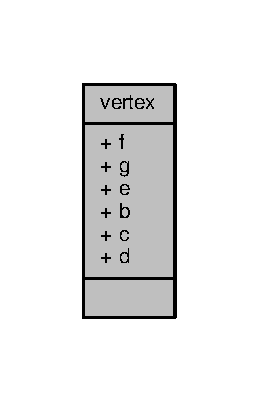
\includegraphics[width=124pt]{structvertex__coll__graph}
\end{center}
\end{figure}
\subsection*{Public Attributes}
\begin{DoxyCompactItemize}
\item 
string \hyperlink{structvertex_a5d46b53771d1b9d8b5cfb6029885e459}{f}
\item 
string \hyperlink{structvertex_a39517d9a99f88564f9df7b769bb6bc03}{g}
\item 
float \hyperlink{structvertex_af8d8ef1d3668f17dd630f21b08e655af}{e}
\item 
float \hyperlink{structvertex_a6df5b4f72e5950da15cdbaca18ac1230}{b}
\item 
float \hyperlink{structvertex_aa81f2ac6178fa638e21e0ffdbe55eeed}{c}
\item 
float \hyperlink{structvertex_a141c5cd092c8ba46392e5f068422f985}{d}
\end{DoxyCompactItemize}


\subsection{Member Data Documentation}
\index{vertex@{vertex}!b@{b}}
\index{b@{b}!vertex@{vertex}}
\subsubsection[{\texorpdfstring{b}{b}}]{\setlength{\rightskip}{0pt plus 5cm}float vertex\+::b}\hypertarget{structvertex_a6df5b4f72e5950da15cdbaca18ac1230}{}\label{structvertex_a6df5b4f72e5950da15cdbaca18ac1230}
\index{vertex@{vertex}!c@{c}}
\index{c@{c}!vertex@{vertex}}
\subsubsection[{\texorpdfstring{c}{c}}]{\setlength{\rightskip}{0pt plus 5cm}float vertex\+::c}\hypertarget{structvertex_aa81f2ac6178fa638e21e0ffdbe55eeed}{}\label{structvertex_aa81f2ac6178fa638e21e0ffdbe55eeed}
\index{vertex@{vertex}!d@{d}}
\index{d@{d}!vertex@{vertex}}
\subsubsection[{\texorpdfstring{d}{d}}]{\setlength{\rightskip}{0pt plus 5cm}float vertex\+::d}\hypertarget{structvertex_a141c5cd092c8ba46392e5f068422f985}{}\label{structvertex_a141c5cd092c8ba46392e5f068422f985}
\index{vertex@{vertex}!e@{e}}
\index{e@{e}!vertex@{vertex}}
\subsubsection[{\texorpdfstring{e}{e}}]{\setlength{\rightskip}{0pt plus 5cm}float vertex\+::e}\hypertarget{structvertex_af8d8ef1d3668f17dd630f21b08e655af}{}\label{structvertex_af8d8ef1d3668f17dd630f21b08e655af}
Two vertices having an edge between them are stored along with their co-\/ordinated(2D). \index{vertex@{vertex}!f@{f}}
\index{f@{f}!vertex@{vertex}}
\subsubsection[{\texorpdfstring{f}{f}}]{\setlength{\rightskip}{0pt plus 5cm}string vertex\+::f}\hypertarget{structvertex_a5d46b53771d1b9d8b5cfb6029885e459}{}\label{structvertex_a5d46b53771d1b9d8b5cfb6029885e459}
\index{vertex@{vertex}!g@{g}}
\index{g@{g}!vertex@{vertex}}
\subsubsection[{\texorpdfstring{g}{g}}]{\setlength{\rightskip}{0pt plus 5cm}string vertex\+::g}\hypertarget{structvertex_a39517d9a99f88564f9df7b769bb6bc03}{}\label{structvertex_a39517d9a99f88564f9df7b769bb6bc03}


The documentation for this struct was generated from the following file\+:\begin{DoxyCompactItemize}
\item 
src/\hyperlink{main_8cpp}{main.\+cpp}\end{DoxyCompactItemize}

\chapter{File Documentation}
\hypertarget{2D__file_8h}{}\section{include/2\+D\+\_\+file.h File Reference}
\label{2D__file_8h}\index{include/2\+D\+\_\+file.\+h@{include/2\+D\+\_\+file.\+h}}
{\ttfamily \#include $<$iostream$>$}\\*
{\ttfamily \#include $<$string$>$}\\*
{\ttfamily \#include $<$vector$>$}\\*
{\ttfamily \#include $<$map$>$}\\*
{\ttfamily \#include $<$math.\+h$>$}\\*
{\ttfamily \#include $<$fstream$>$}\\*
{\ttfamily \#include \char`\"{}graph.\+h\char`\"{}}\\*
Include dependency graph for 2\+D\+\_\+file.h\+:
\nopagebreak
\begin{figure}[H]
\begin{center}
\leavevmode
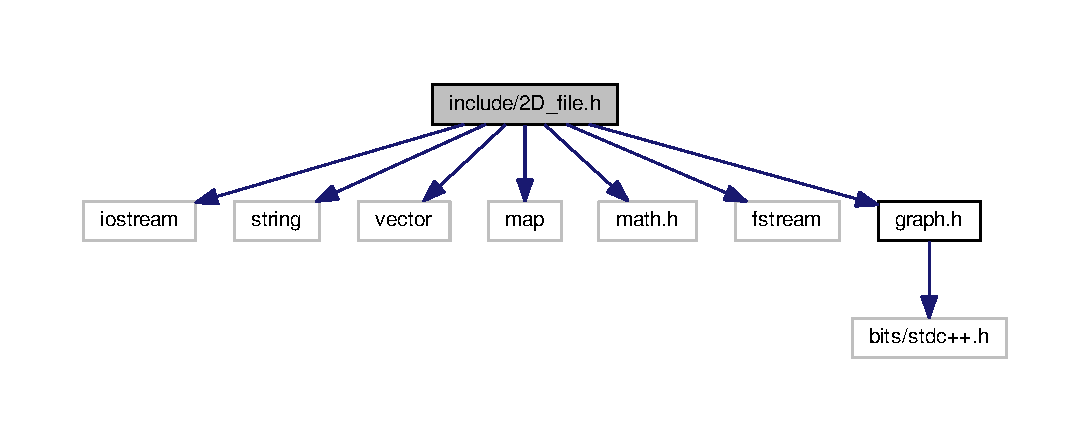
\includegraphics[width=350pt]{2D__file_8h__incl}
\end{center}
\end{figure}
This graph shows which files directly or indirectly include this file\+:
\nopagebreak
\begin{figure}[H]
\begin{center}
\leavevmode
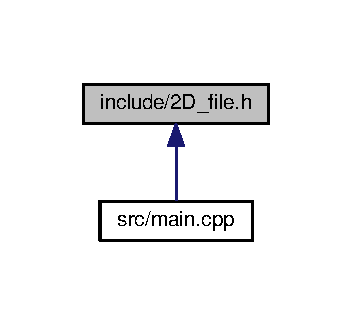
\includegraphics[width=169pt]{2D__file_8h__dep__incl}
\end{center}
\end{figure}
\subsection*{Macros}
\begin{DoxyCompactItemize}
\item 
\#define \hyperlink{2D__file_8h_a7988c4ca31adb885a06ee851c72a59e7}{\+\_\+\+\_\+\+A\+P\+\_\+\+\_\+}
\end{DoxyCompactItemize}
\subsection*{Functions}
\begin{DoxyCompactItemize}
\item 
void \hyperlink{2D__file_8h_ab70fe8e1ebd76273def62d68c8360b6a}{tokenize} (string a, vector$<$ string $>$ \&vect)
\item 
string \hyperlink{2D__file_8h_a9c53af81dab2b1850b3f7b717610d0a7}{get\+\_\+2\+D\+\_\+graph} (vector$<$ vector$<$ \hyperlink{structco__ordinates__2D}{co\+\_\+ordinates\+\_\+2D} $>$ $>$ \&cz, vector$<$ string $>$ \&edges1, vector$<$ string $>$ \&edges2, vector$<$ string $>$ \&edges3)
\end{DoxyCompactItemize}


\subsection{Macro Definition Documentation}
\index{2\+D\+\_\+file.\+h@{2\+D\+\_\+file.\+h}!\+\_\+\+\_\+\+A\+P\+\_\+\+\_\+@{\+\_\+\+\_\+\+A\+P\+\_\+\+\_\+}}
\index{\+\_\+\+\_\+\+A\+P\+\_\+\+\_\+@{\+\_\+\+\_\+\+A\+P\+\_\+\+\_\+}!2\+D\+\_\+file.\+h@{2\+D\+\_\+file.\+h}}
\subsubsection[{\texorpdfstring{\+\_\+\+\_\+\+A\+P\+\_\+\+\_\+}{__AP__}}]{\setlength{\rightskip}{0pt plus 5cm}\#define \+\_\+\+\_\+\+A\+P\+\_\+\+\_\+}\hypertarget{2D__file_8h_a7988c4ca31adb885a06ee851c72a59e7}{}\label{2D__file_8h_a7988c4ca31adb885a06ee851c72a59e7}


\subsection{Function Documentation}
\index{2\+D\+\_\+file.\+h@{2\+D\+\_\+file.\+h}!get\+\_\+2\+D\+\_\+graph@{get\+\_\+2\+D\+\_\+graph}}
\index{get\+\_\+2\+D\+\_\+graph@{get\+\_\+2\+D\+\_\+graph}!2\+D\+\_\+file.\+h@{2\+D\+\_\+file.\+h}}
\subsubsection[{\texorpdfstring{get\+\_\+2\+D\+\_\+graph(vector$<$ vector$<$ co\+\_\+ordinates\+\_\+2\+D $>$ $>$ \&cz, vector$<$ string $>$ \&edges1, vector$<$ string $>$ \&edges2, vector$<$ string $>$ \&edges3)}{get_2D_graph(vector< vector< co_ordinates_2D > > &cz, vector< string > &edges1, vector< string > &edges2, vector< string > &edges3)}}]{\setlength{\rightskip}{0pt plus 5cm}string get\+\_\+2\+D\+\_\+graph (
\begin{DoxyParamCaption}
\item[{vector$<$ vector$<$ {\bf co\+\_\+ordinates\+\_\+2D} $>$ $>$ \&}]{cz, }
\item[{vector$<$ string $>$ \&}]{edges1, }
\item[{vector$<$ string $>$ \&}]{edges2, }
\item[{vector$<$ string $>$ \&}]{edges3}
\end{DoxyParamCaption}
)}\hypertarget{2D__file_8h_a9c53af81dab2b1850b3f7b717610d0a7}{}\label{2D__file_8h_a9c53af81dab2b1850b3f7b717610d0a7}
\index{2\+D\+\_\+file.\+h@{2\+D\+\_\+file.\+h}!tokenize@{tokenize}}
\index{tokenize@{tokenize}!2\+D\+\_\+file.\+h@{2\+D\+\_\+file.\+h}}
\subsubsection[{\texorpdfstring{tokenize(string a, vector$<$ string $>$ \&vect)}{tokenize(string a, vector< string > &vect)}}]{\setlength{\rightskip}{0pt plus 5cm}void tokenize (
\begin{DoxyParamCaption}
\item[{string}]{a, }
\item[{vector$<$ string $>$ \&}]{vect}
\end{DoxyParamCaption}
)}\hypertarget{2D__file_8h_ab70fe8e1ebd76273def62d68c8360b6a}{}\label{2D__file_8h_ab70fe8e1ebd76273def62d68c8360b6a}

\hypertarget{3D__file_8h}{}\section{include/3\+D\+\_\+file.h File Reference}
\label{3D__file_8h}\index{include/3\+D\+\_\+file.\+h@{include/3\+D\+\_\+file.\+h}}
{\ttfamily \#include $<$iostream$>$}\\*
{\ttfamily \#include $<$string$>$}\\*
{\ttfamily \#include $<$vector$>$}\\*
{\ttfamily \#include $<$map$>$}\\*
{\ttfamily \#include $<$fstream$>$}\\*
{\ttfamily \#include $<$math.\+h$>$}\\*
{\ttfamily \#include \char`\"{}graph.\+h\char`\"{}}\\*
Include dependency graph for 3\+D\+\_\+file.h\+:
\nopagebreak
\begin{figure}[H]
\begin{center}
\leavevmode
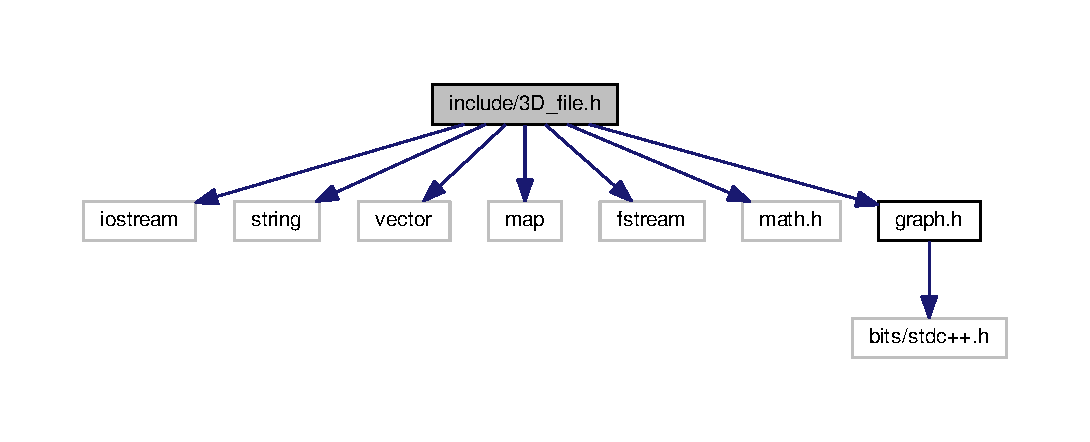
\includegraphics[width=350pt]{3D__file_8h__incl}
\end{center}
\end{figure}
This graph shows which files directly or indirectly include this file\+:
\nopagebreak
\begin{figure}[H]
\begin{center}
\leavevmode
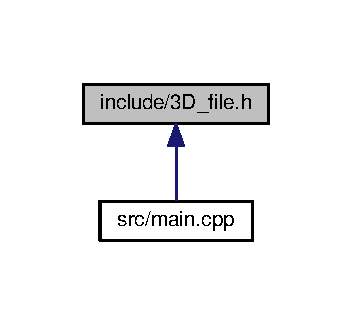
\includegraphics[width=169pt]{3D__file_8h__dep__incl}
\end{center}
\end{figure}
\subsection*{Functions}
\begin{DoxyCompactItemize}
\item 
string \hyperlink{3D__file_8h_a4678459e35018e5cd5a3e77751c90430}{get\+\_\+3\+D\+\_\+graph} (vector$<$ \hyperlink{structco__ordinates__3D}{co\+\_\+ordinates\+\_\+3D} $>$ \&c, vector$<$ string $>$ \&faces)
\end{DoxyCompactItemize}


\subsection{Function Documentation}
\index{3\+D\+\_\+file.\+h@{3\+D\+\_\+file.\+h}!get\+\_\+3\+D\+\_\+graph@{get\+\_\+3\+D\+\_\+graph}}
\index{get\+\_\+3\+D\+\_\+graph@{get\+\_\+3\+D\+\_\+graph}!3\+D\+\_\+file.\+h@{3\+D\+\_\+file.\+h}}
\subsubsection[{\texorpdfstring{get\+\_\+3\+D\+\_\+graph(vector$<$ co\+\_\+ordinates\+\_\+3\+D $>$ \&c, vector$<$ string $>$ \&faces)}{get_3D_graph(vector< co_ordinates_3D > &c, vector< string > &faces)}}]{\setlength{\rightskip}{0pt plus 5cm}string get\+\_\+3\+D\+\_\+graph (
\begin{DoxyParamCaption}
\item[{vector$<$ {\bf co\+\_\+ordinates\+\_\+3D} $>$ \&}]{c, }
\item[{vector$<$ string $>$ \&}]{faces}
\end{DoxyParamCaption}
)}\hypertarget{3D__file_8h_a4678459e35018e5cd5a3e77751c90430}{}\label{3D__file_8h_a4678459e35018e5cd5a3e77751c90430}

\hypertarget{conversion_8h}{}\section{include/conversion.h File Reference}
\label{conversion_8h}\index{include/conversion.\+h@{include/conversion.\+h}}
{\ttfamily \#include $<$iostream$>$}\\*
{\ttfamily \#include $<$string$>$}\\*
{\ttfamily \#include $<$vector$>$}\\*
{\ttfamily \#include $<$map$>$}\\*
{\ttfamily \#include $<$fstream$>$}\\*
{\ttfamily \#include $<$math.\+h$>$}\\*
{\ttfamily \#include \char`\"{}graph.\+h\char`\"{}}\\*
Include dependency graph for conversion.\+h\+:
\nopagebreak
\begin{figure}[H]
\begin{center}
\leavevmode
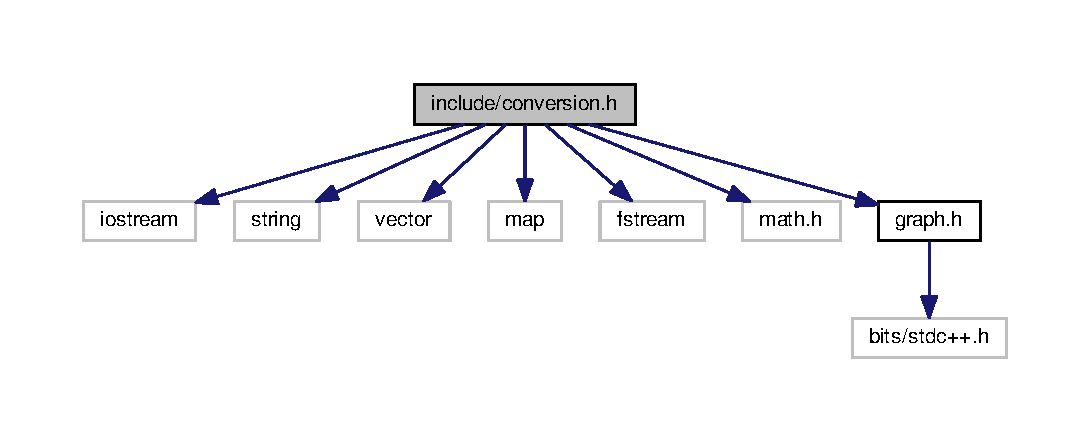
\includegraphics[width=350pt]{conversion_8h__incl}
\end{center}
\end{figure}
This graph shows which files directly or indirectly include this file\+:
\nopagebreak
\begin{figure}[H]
\begin{center}
\leavevmode
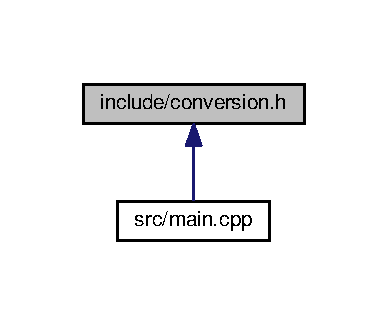
\includegraphics[width=186pt]{conversion_8h__dep__incl}
\end{center}
\end{figure}
\subsection*{Functions}
\begin{DoxyCompactItemize}
\item 
void \hyperlink{conversion_8h_a2169682c30246c37ce36a800ed684c65}{tokenize1} (string a, vector$<$ string $>$ \&vect)
\item 
void \hyperlink{conversion_8h_abebdd35624d5eeabe7862422d2bff335}{isometric} (vector$<$ vector$<$ \hyperlink{structco__ordinates__2D}{co\+\_\+ordinates\+\_\+2D} $>$ $>$ outgraphs2, vector$<$ string $>$ edges1, vector$<$ string $>$ edges2, vector$<$ string $>$ edges3)
\end{DoxyCompactItemize}


\subsection{Function Documentation}
\index{conversion.\+h@{conversion.\+h}!isometric@{isometric}}
\index{isometric@{isometric}!conversion.\+h@{conversion.\+h}}
\subsubsection[{\texorpdfstring{isometric(vector$<$ vector$<$ co\+\_\+ordinates\+\_\+2\+D $>$ $>$ outgraphs2, vector$<$ string $>$ edges1, vector$<$ string $>$ edges2, vector$<$ string $>$ edges3)}{isometric(vector< vector< co_ordinates_2D > > outgraphs2, vector< string > edges1, vector< string > edges2, vector< string > edges3)}}]{\setlength{\rightskip}{0pt plus 5cm}void isometric (
\begin{DoxyParamCaption}
\item[{vector$<$ vector$<$ {\bf co\+\_\+ordinates\+\_\+2D} $>$ $>$}]{outgraphs2, }
\item[{vector$<$ string $>$}]{edges1, }
\item[{vector$<$ string $>$}]{edges2, }
\item[{vector$<$ string $>$}]{edges3}
\end{DoxyParamCaption}
)}\hypertarget{conversion_8h_abebdd35624d5eeabe7862422d2bff335}{}\label{conversion_8h_abebdd35624d5eeabe7862422d2bff335}
\index{conversion.\+h@{conversion.\+h}!tokenize1@{tokenize1}}
\index{tokenize1@{tokenize1}!conversion.\+h@{conversion.\+h}}
\subsubsection[{\texorpdfstring{tokenize1(string a, vector$<$ string $>$ \&vect)}{tokenize1(string a, vector< string > &vect)}}]{\setlength{\rightskip}{0pt plus 5cm}void tokenize1 (
\begin{DoxyParamCaption}
\item[{string}]{a, }
\item[{vector$<$ string $>$ \&}]{vect}
\end{DoxyParamCaption}
)}\hypertarget{conversion_8h_a2169682c30246c37ce36a800ed684c65}{}\label{conversion_8h_a2169682c30246c37ce36a800ed684c65}

\hypertarget{file__3D__temp_8h}{}\section{include/file\+\_\+3\+D\+\_\+temp.h File Reference}
\label{file__3D__temp_8h}\index{include/file\+\_\+3\+D\+\_\+temp.\+h@{include/file\+\_\+3\+D\+\_\+temp.\+h}}
{\ttfamily \#include $<$iostream$>$}\\*
{\ttfamily \#include $<$string$>$}\\*
{\ttfamily \#include $<$vector$>$}\\*
{\ttfamily \#include $<$map$>$}\\*
{\ttfamily \#include $<$math.\+h$>$}\\*
{\ttfamily \#include $<$fstream$>$}\\*
{\ttfamily \#include $<$Qt\+Core$>$}\\*
{\ttfamily \#include $<$Qt\+Gui$>$}\\*
{\ttfamily \#include $<$Q\+String$>$}\\*
{\ttfamily \#include \char`\"{}graph.\+h\char`\"{}}\\*
Include dependency graph for file\+\_\+3\+D\+\_\+temp.\+h\+:
\nopagebreak
\begin{figure}[H]
\begin{center}
\leavevmode
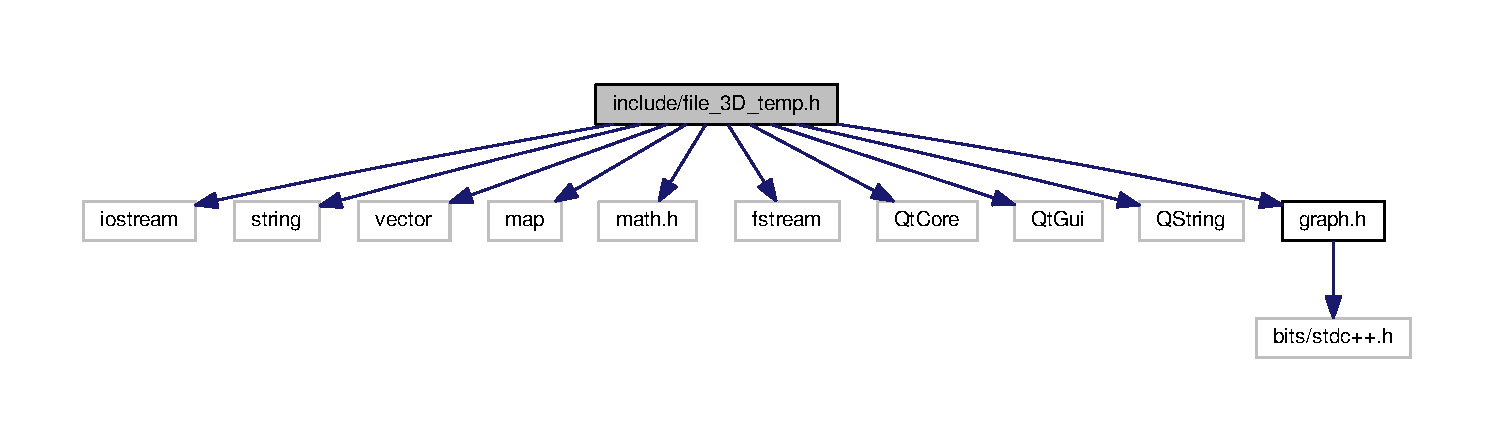
\includegraphics[width=350pt]{file__3D__temp_8h__incl}
\end{center}
\end{figure}
This graph shows which files directly or indirectly include this file\+:
\nopagebreak
\begin{figure}[H]
\begin{center}
\leavevmode
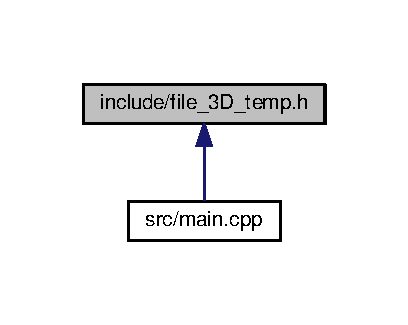
\includegraphics[width=196pt]{file__3D__temp_8h__dep__incl}
\end{center}
\end{figure}
\subsection*{Functions}
\begin{DoxyCompactItemize}
\item 
void \hyperlink{file__3D__temp_8h_a080b3ca0ed76871211ba630eccca780f}{write\+\_\+in\+\_\+out\+\_\+file} (vector$<$ vector$<$ \hyperlink{structco__ordinates__2D}{co\+\_\+ordinates\+\_\+2D} $>$ $>$ outgraphs, int choice)
\end{DoxyCompactItemize}


\subsection{Function Documentation}
\index{file\+\_\+3\+D\+\_\+temp.\+h@{file\+\_\+3\+D\+\_\+temp.\+h}!write\+\_\+in\+\_\+out\+\_\+file@{write\+\_\+in\+\_\+out\+\_\+file}}
\index{write\+\_\+in\+\_\+out\+\_\+file@{write\+\_\+in\+\_\+out\+\_\+file}!file\+\_\+3\+D\+\_\+temp.\+h@{file\+\_\+3\+D\+\_\+temp.\+h}}
\subsubsection[{\texorpdfstring{write\+\_\+in\+\_\+out\+\_\+file(vector$<$ vector$<$ co\+\_\+ordinates\+\_\+2\+D $>$ $>$ outgraphs, int choice)}{write_in_out_file(vector< vector< co_ordinates_2D > > outgraphs, int choice)}}]{\setlength{\rightskip}{0pt plus 5cm}void write\+\_\+in\+\_\+out\+\_\+file (
\begin{DoxyParamCaption}
\item[{vector$<$ vector$<$ {\bf co\+\_\+ordinates\+\_\+2D} $>$ $>$}]{outgraphs, }
\item[{int}]{choice}
\end{DoxyParamCaption}
)}\hypertarget{file__3D__temp_8h_a080b3ca0ed76871211ba630eccca780f}{}\label{file__3D__temp_8h_a080b3ca0ed76871211ba630eccca780f}

\hypertarget{graph_8h}{}\section{include/graph.h File Reference}
\label{graph_8h}\index{include/graph.\+h@{include/graph.\+h}}
{\ttfamily \#include $<$bits/stdc++.\+h$>$}\\*
Include dependency graph for graph.\+h\+:
\nopagebreak
\begin{figure}[H]
\begin{center}
\leavevmode
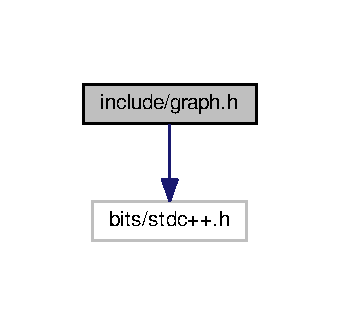
\includegraphics[width=163pt]{graph_8h__incl}
\end{center}
\end{figure}
This graph shows which files directly or indirectly include this file\+:
\nopagebreak
\begin{figure}[H]
\begin{center}
\leavevmode
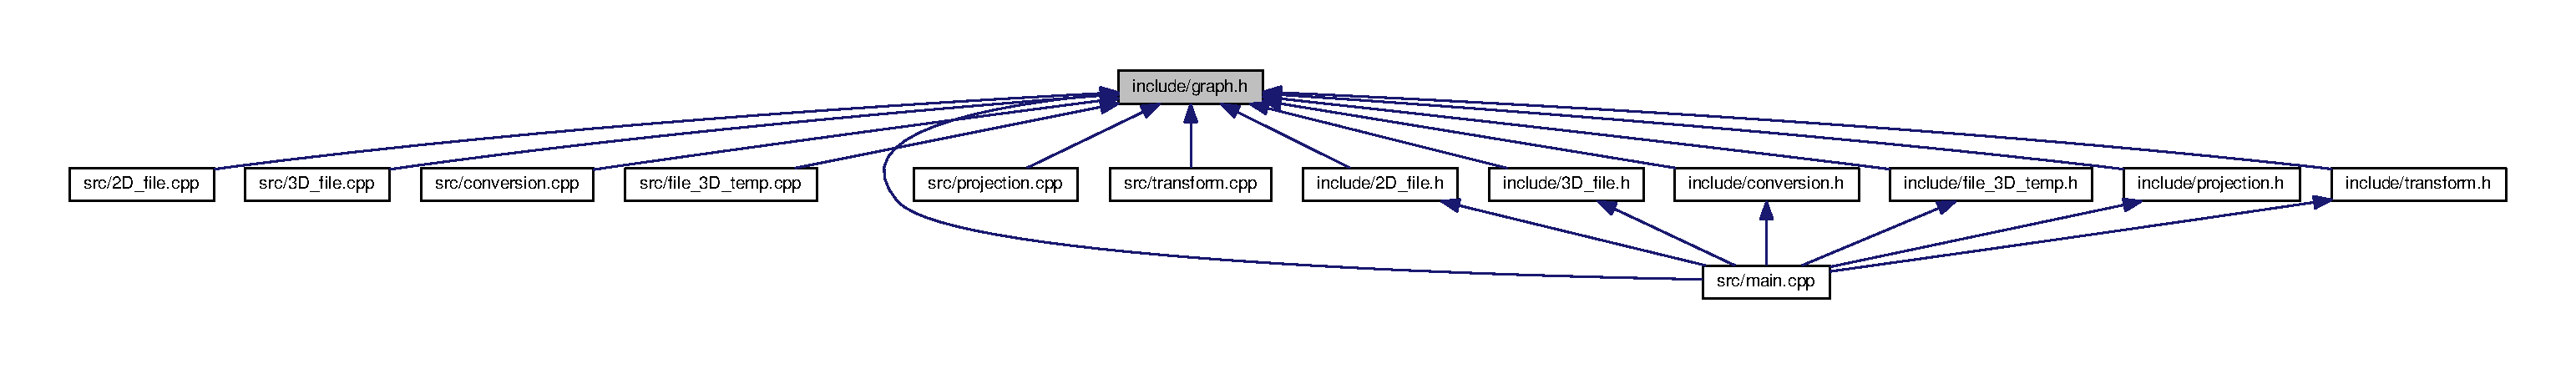
\includegraphics[width=350pt]{graph_8h__dep__incl}
\end{center}
\end{figure}
\subsection*{Classes}
\begin{DoxyCompactItemize}
\item 
struct \hyperlink{structco__ordinates__3D}{co\+\_\+ordinates\+\_\+3D}
\item 
struct \hyperlink{structco__ordinates__2D}{co\+\_\+ordinates\+\_\+2D}
\end{DoxyCompactItemize}

\hypertarget{projection_8h}{}\section{include/projection.h File Reference}
\label{projection_8h}\index{include/projection.\+h@{include/projection.\+h}}
{\ttfamily \#include $<$iostream$>$}\\*
{\ttfamily \#include $<$string$>$}\\*
{\ttfamily \#include $<$vector$>$}\\*
{\ttfamily \#include $<$math.\+h$>$}\\*
{\ttfamily \#include $<$map$>$}\\*
{\ttfamily \#include $<$fstream$>$}\\*
{\ttfamily \#include \char`\"{}graph.\+h\char`\"{}}\\*
Include dependency graph for projection.\+h\+:
\nopagebreak
\begin{figure}[H]
\begin{center}
\leavevmode
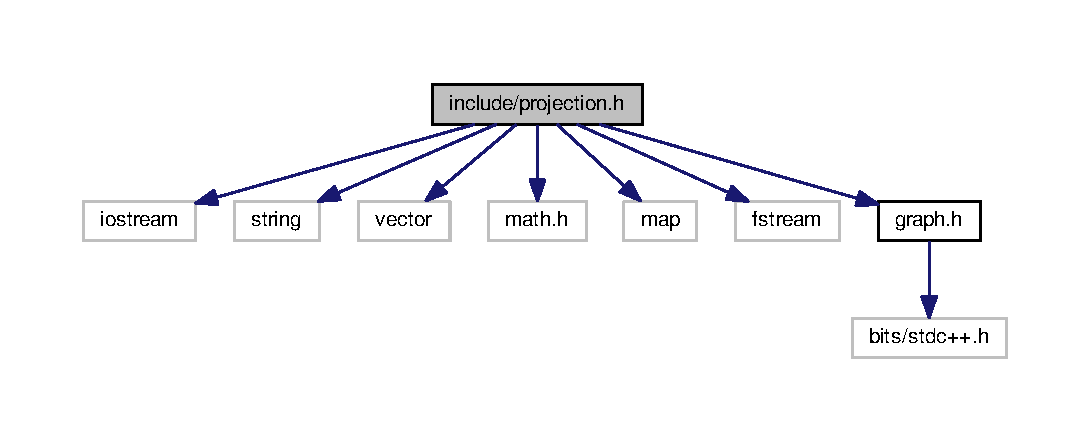
\includegraphics[width=350pt]{projection_8h__incl}
\end{center}
\end{figure}
This graph shows which files directly or indirectly include this file\+:
\nopagebreak
\begin{figure}[H]
\begin{center}
\leavevmode
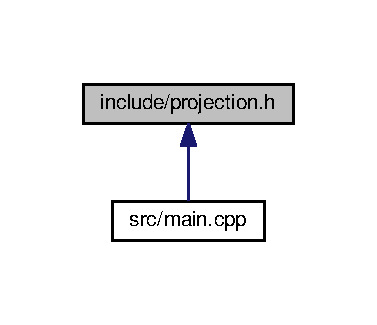
\includegraphics[width=181pt]{projection_8h__dep__incl}
\end{center}
\end{figure}
\subsection*{Functions}
\begin{DoxyCompactItemize}
\item 
void \hyperlink{projection_8h_ac09069ee10271e589ccdaa86b67fc33f}{projections} (vector$<$ \hyperlink{structco__ordinates__3D}{co\+\_\+ordinates\+\_\+3D} $>$ \&c, vector$<$ vector$<$ \hyperlink{structco__ordinates__2D}{co\+\_\+ordinates\+\_\+2D} $>$ $>$ \&graphs)
\end{DoxyCompactItemize}


\subsection{Function Documentation}
\index{projection.\+h@{projection.\+h}!projections@{projections}}
\index{projections@{projections}!projection.\+h@{projection.\+h}}
\subsubsection[{\texorpdfstring{projections(vector$<$ co\+\_\+ordinates\+\_\+3\+D $>$ \&c, vector$<$ vector$<$ co\+\_\+ordinates\+\_\+2\+D $>$ $>$ \&graphs)}{projections(vector< co_ordinates_3D > &c, vector< vector< co_ordinates_2D > > &graphs)}}]{\setlength{\rightskip}{0pt plus 5cm}void projections (
\begin{DoxyParamCaption}
\item[{vector$<$ {\bf co\+\_\+ordinates\+\_\+3D} $>$ \&}]{c, }
\item[{vector$<$ vector$<$ {\bf co\+\_\+ordinates\+\_\+2D} $>$ $>$ \&}]{graphs}
\end{DoxyParamCaption}
)}\hypertarget{projection_8h_ac09069ee10271e589ccdaa86b67fc33f}{}\label{projection_8h_ac09069ee10271e589ccdaa86b67fc33f}

\hypertarget{transform_8h}{}\section{include/transform.h File Reference}
\label{transform_8h}\index{include/transform.\+h@{include/transform.\+h}}
{\ttfamily \#include $<$iostream$>$}\\*
{\ttfamily \#include $<$string$>$}\\*
{\ttfamily \#include $<$vector$>$}\\*
{\ttfamily \#include $<$math.\+h$>$}\\*
{\ttfamily \#include \char`\"{}graph.\+h\char`\"{}}\\*
Include dependency graph for transform.\+h\+:
\nopagebreak
\begin{figure}[H]
\begin{center}
\leavevmode
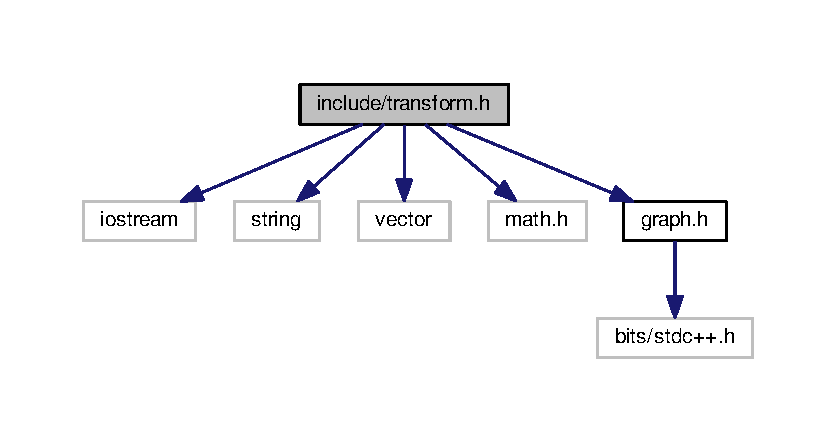
\includegraphics[width=350pt]{transform_8h__incl}
\end{center}
\end{figure}
This graph shows which files directly or indirectly include this file\+:
\nopagebreak
\begin{figure}[H]
\begin{center}
\leavevmode
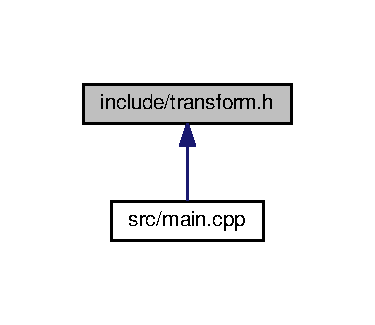
\includegraphics[width=180pt]{transform_8h__dep__incl}
\end{center}
\end{figure}
\subsection*{Functions}
\begin{DoxyCompactItemize}
\item 
int \hyperlink{transform_8h_ad2538d9d4e11957051c02a3e8f5fd2f4}{transform} (vector$<$ \hyperlink{structco__ordinates__3D}{co\+\_\+ordinates\+\_\+3D} $>$ \&graph, vector$<$ string $>$ faces, vector$<$ string $>$ \&points)
\end{DoxyCompactItemize}


\subsection{Function Documentation}
\index{transform.\+h@{transform.\+h}!transform@{transform}}
\index{transform@{transform}!transform.\+h@{transform.\+h}}
\subsubsection[{\texorpdfstring{transform(vector$<$ co\+\_\+ordinates\+\_\+3\+D $>$ \&graph, vector$<$ string $>$ faces, vector$<$ string $>$ \&points)}{transform(vector< co_ordinates_3D > &graph, vector< string > faces, vector< string > &points)}}]{\setlength{\rightskip}{0pt plus 5cm}int transform (
\begin{DoxyParamCaption}
\item[{vector$<$ {\bf co\+\_\+ordinates\+\_\+3D} $>$ \&}]{graph, }
\item[{vector$<$ string $>$}]{faces, }
\item[{vector$<$ string $>$ \&}]{points}
\end{DoxyParamCaption}
)}\hypertarget{transform_8h_ad2538d9d4e11957051c02a3e8f5fd2f4}{}\label{transform_8h_ad2538d9d4e11957051c02a3e8f5fd2f4}

\hypertarget{2D__file_8cpp}{}\section{src/2\+D\+\_\+file.cpp File Reference}
\label{2D__file_8cpp}\index{src/2\+D\+\_\+file.\+cpp@{src/2\+D\+\_\+file.\+cpp}}
{\ttfamily \#include $<$iostream$>$}\\*
{\ttfamily \#include $<$string$>$}\\*
{\ttfamily \#include $<$vector$>$}\\*
{\ttfamily \#include $<$map$>$}\\*
{\ttfamily \#include $<$fstream$>$}\\*
{\ttfamily \#include $<$math.\+h$>$}\\*
{\ttfamily \#include \char`\"{}graph.\+h\char`\"{}}\\*
Include dependency graph for 2\+D\+\_\+file.cpp\+:
\nopagebreak
\begin{figure}[H]
\begin{center}
\leavevmode
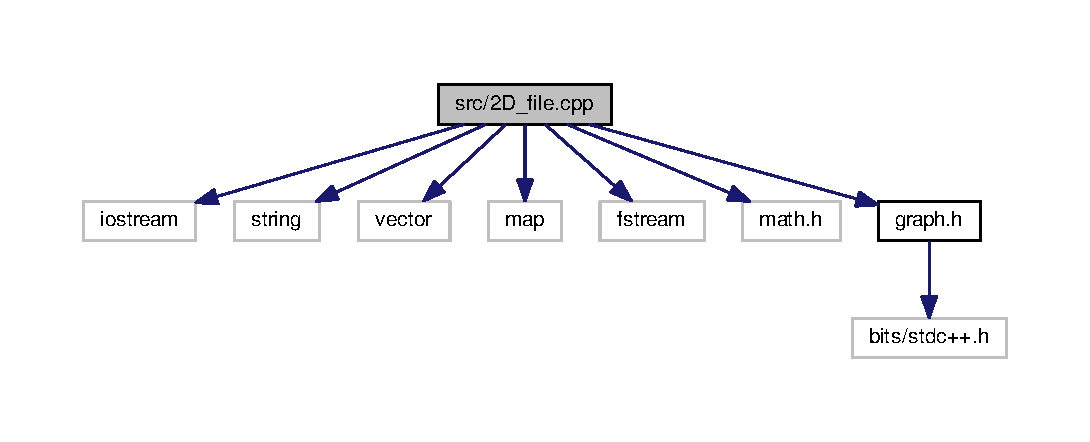
\includegraphics[width=350pt]{2D__file_8cpp__incl}
\end{center}
\end{figure}
\subsection*{Classes}
\begin{DoxyCompactItemize}
\item 
class \hyperlink{class__2D__file}{\+\_\+2\+D\+\_\+file}
\end{DoxyCompactItemize}

\hypertarget{3D__file_8cpp}{}\section{src/3\+D\+\_\+file.cpp File Reference}
\label{3D__file_8cpp}\index{src/3\+D\+\_\+file.\+cpp@{src/3\+D\+\_\+file.\+cpp}}
{\ttfamily \#include $<$iostream$>$}\\*
{\ttfamily \#include $<$string$>$}\\*
{\ttfamily \#include $<$vector$>$}\\*
{\ttfamily \#include $<$map$>$}\\*
{\ttfamily \#include $<$fstream$>$}\\*
{\ttfamily \#include $<$math.\+h$>$}\\*
{\ttfamily \#include \char`\"{}graph.\+h\char`\"{}}\\*
Include dependency graph for 3\+D\+\_\+file.cpp\+:
\nopagebreak
\begin{figure}[H]
\begin{center}
\leavevmode
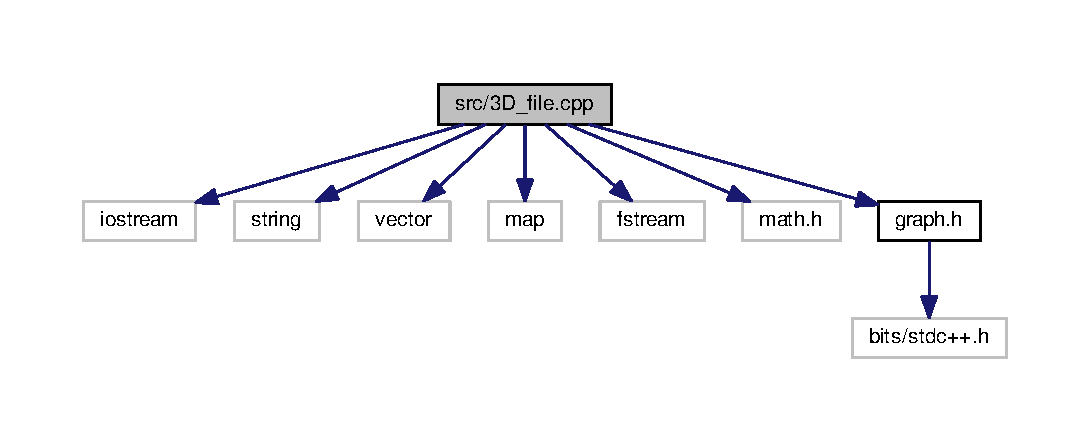
\includegraphics[width=350pt]{3D__file_8cpp__incl}
\end{center}
\end{figure}
\subsection*{Classes}
\begin{DoxyCompactItemize}
\item 
class \hyperlink{class__3D__file}{\+\_\+3\+D\+\_\+file}
\end{DoxyCompactItemize}

\hypertarget{conversion_8cpp}{}\section{src/conversion.cpp File Reference}
\label{conversion_8cpp}\index{src/conversion.\+cpp@{src/conversion.\+cpp}}
{\ttfamily \#include $<$iostream$>$}\\*
{\ttfamily \#include $<$string$>$}\\*
{\ttfamily \#include $<$vector$>$}\\*
{\ttfamily \#include $<$map$>$}\\*
{\ttfamily \#include $<$fstream$>$}\\*
{\ttfamily \#include $<$math.\+h$>$}\\*
{\ttfamily \#include \char`\"{}graph.\+h\char`\"{}}\\*
Include dependency graph for conversion.\+cpp\+:
\nopagebreak
\begin{figure}[H]
\begin{center}
\leavevmode
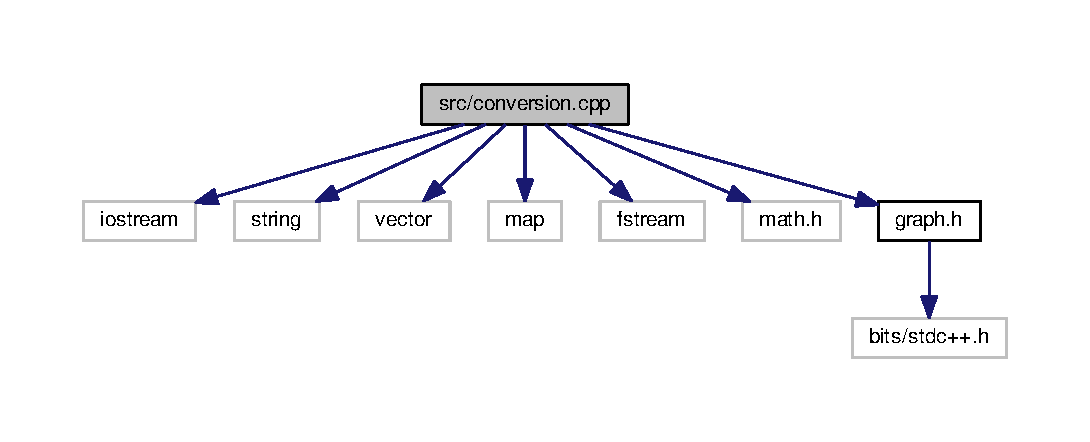
\includegraphics[width=350pt]{conversion_8cpp__incl}
\end{center}
\end{figure}
\subsection*{Classes}
\begin{DoxyCompactItemize}
\item 
class \hyperlink{classconversion}{conversion}
\end{DoxyCompactItemize}

\hypertarget{file__3D__temp_8cpp}{}\section{src/file\+\_\+3\+D\+\_\+temp.cpp File Reference}
\label{file__3D__temp_8cpp}\index{src/file\+\_\+3\+D\+\_\+temp.\+cpp@{src/file\+\_\+3\+D\+\_\+temp.\+cpp}}
{\ttfamily \#include $<$iostream$>$}\\*
{\ttfamily \#include $<$string$>$}\\*
{\ttfamily \#include $<$vector$>$}\\*
{\ttfamily \#include $<$map$>$}\\*
{\ttfamily \#include $<$math.\+h$>$}\\*
{\ttfamily \#include $<$fstream$>$}\\*
{\ttfamily \#include \char`\"{}graph.\+h\char`\"{}}\\*
Include dependency graph for file\+\_\+3\+D\+\_\+temp.\+cpp\+:
\nopagebreak
\begin{figure}[H]
\begin{center}
\leavevmode
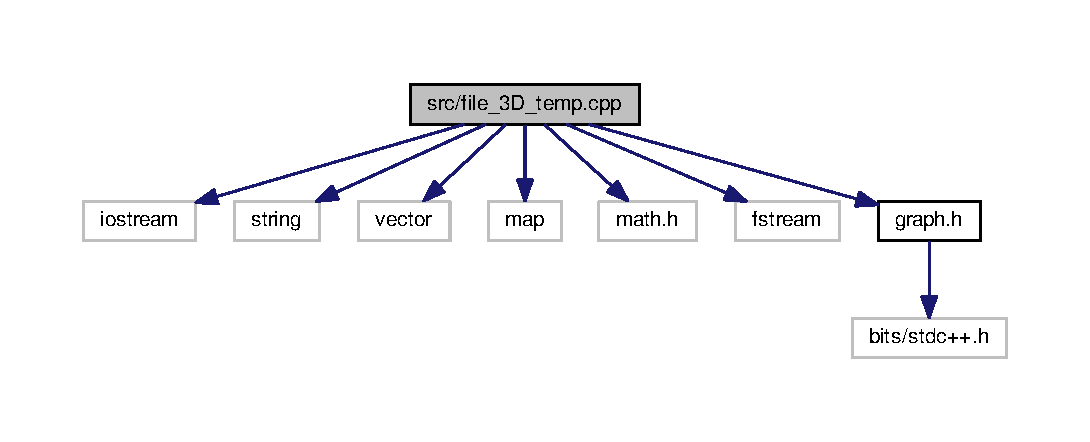
\includegraphics[width=350pt]{file__3D__temp_8cpp__incl}
\end{center}
\end{figure}
\subsection*{Classes}
\begin{DoxyCompactItemize}
\item 
class \hyperlink{classfile__3D__temp}{file\+\_\+3\+D\+\_\+temp}
\end{DoxyCompactItemize}

\hypertarget{main_8cpp}{}\section{src/main.cpp File Reference}
\label{main_8cpp}\index{src/main.\+cpp@{src/main.\+cpp}}
{\ttfamily \#include $<$math.\+h$>$}\\*
{\ttfamily \#include $<$Qt\+Core$>$}\\*
{\ttfamily \#include $<$Qt\+Gui$>$}\\*
{\ttfamily \#include $<$Q\+String$>$}\\*
{\ttfamily \#include $<$iostream$>$}\\*
{\ttfamily \#include $<$string$>$}\\*
{\ttfamily \#include $<$vector$>$}\\*
{\ttfamily \#include $<$fstream$>$}\\*
{\ttfamily \#include $<$map$>$}\\*
{\ttfamily \#include \char`\"{}transform.\+h\char`\"{}}\\*
{\ttfamily \#include \char`\"{}2\+D\+\_\+file.\+h\char`\"{}}\\*
{\ttfamily \#include \char`\"{}graph.\+h\char`\"{}}\\*
{\ttfamily \#include \char`\"{}conversion.\+h\char`\"{}}\\*
{\ttfamily \#include \char`\"{}file\+\_\+3\+D\+\_\+temp.\+h\char`\"{}}\\*
{\ttfamily \#include \char`\"{}projection.\+h\char`\"{}}\\*
{\ttfamily \#include \char`\"{}3\+D\+\_\+file.\+h\char`\"{}}\\*
Include dependency graph for main.\+cpp\+:
\nopagebreak
\begin{figure}[H]
\begin{center}
\leavevmode
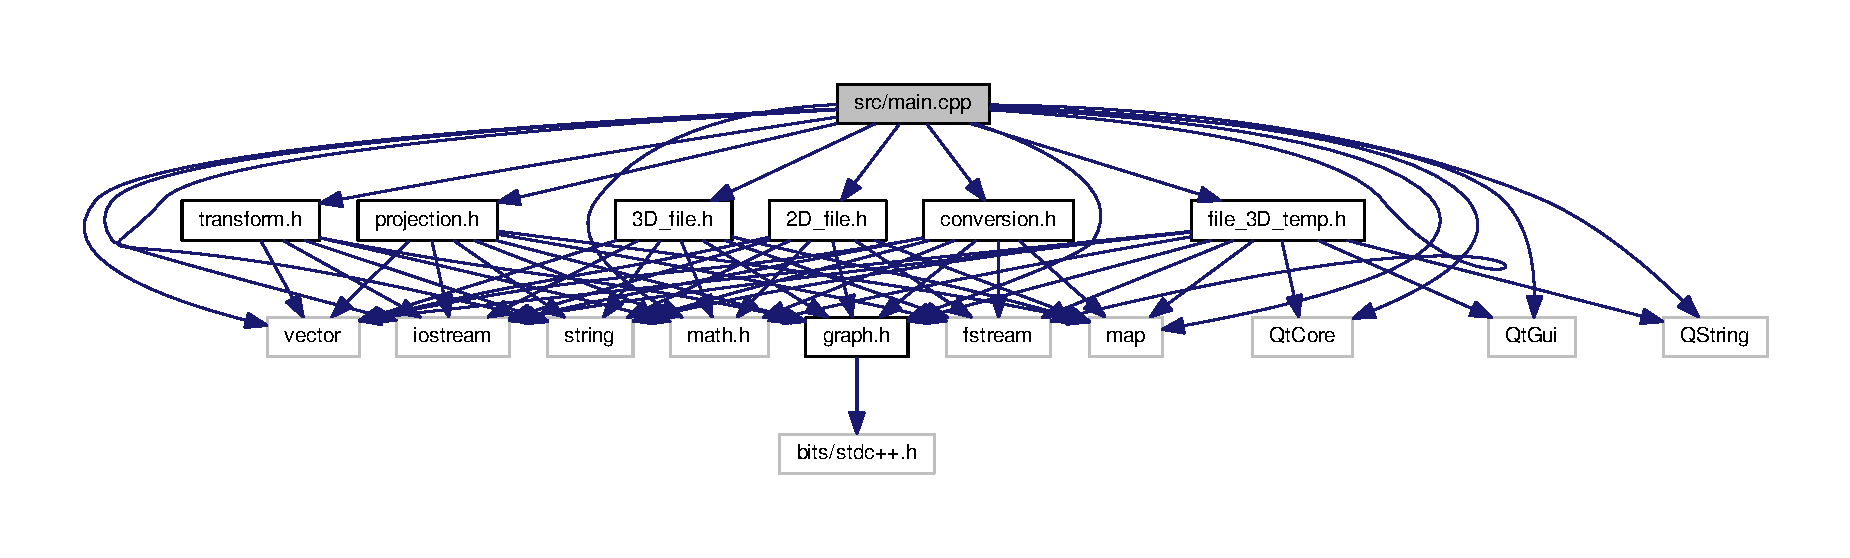
\includegraphics[width=350pt]{main_8cpp__incl}
\end{center}
\end{figure}
\subsection*{Classes}
\begin{DoxyCompactItemize}
\item 
struct \hyperlink{structvertex}{vertex}
\item 
class \hyperlink{classMaster}{Master}
\end{DoxyCompactItemize}
\subsection*{Macros}
\begin{DoxyCompactItemize}
\item 
\#define \hyperlink{main_8cpp_a598a3330b3c21701223ee0ca14316eca}{PI}~3.\+1415926536
\end{DoxyCompactItemize}


\subsection{Macro Definition Documentation}
\index{main.\+cpp@{main.\+cpp}!PI@{PI}}
\index{PI@{PI}!main.\+cpp@{main.\+cpp}}
\subsubsection[{\texorpdfstring{PI}{PI}}]{\setlength{\rightskip}{0pt plus 5cm}\#define PI~3.\+1415926536}\hypertarget{main_8cpp_a598a3330b3c21701223ee0ca14316eca}{}\label{main_8cpp_a598a3330b3c21701223ee0ca14316eca}

\hypertarget{projection_8cpp}{}\section{src/projection.cpp File Reference}
\label{projection_8cpp}\index{src/projection.\+cpp@{src/projection.\+cpp}}
{\ttfamily \#include $<$iostream$>$}\\*
{\ttfamily \#include $<$string$>$}\\*
{\ttfamily \#include $<$vector$>$}\\*
{\ttfamily \#include $<$math.\+h$>$}\\*
{\ttfamily \#include $<$fstream$>$}\\*
{\ttfamily \#include \char`\"{}graph.\+h\char`\"{}}\\*
Include dependency graph for projection.\+cpp\+:
\nopagebreak
\begin{figure}[H]
\begin{center}
\leavevmode
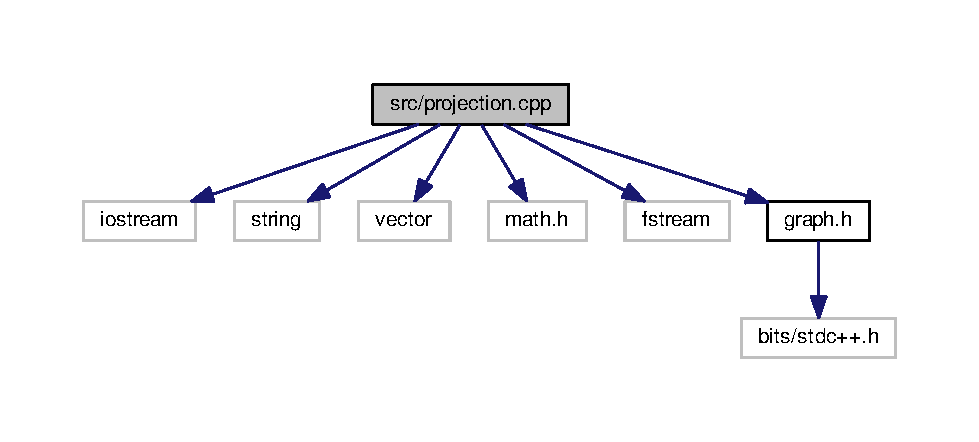
\includegraphics[width=350pt]{projection_8cpp__incl}
\end{center}
\end{figure}
\subsection*{Classes}
\begin{DoxyCompactItemize}
\item 
class \hyperlink{classprojection}{projection}
\end{DoxyCompactItemize}

\hypertarget{transform_8cpp}{}\section{src/transform.cpp File Reference}
\label{transform_8cpp}\index{src/transform.\+cpp@{src/transform.\+cpp}}
{\ttfamily \#include $<$iostream$>$}\\*
{\ttfamily \#include $<$string$>$}\\*
{\ttfamily \#include $<$vector$>$}\\*
{\ttfamily \#include $<$math.\+h$>$}\\*
{\ttfamily \#include \char`\"{}graph.\+h\char`\"{}}\\*
Include dependency graph for transform.\+cpp\+:
\nopagebreak
\begin{figure}[H]
\begin{center}
\leavevmode
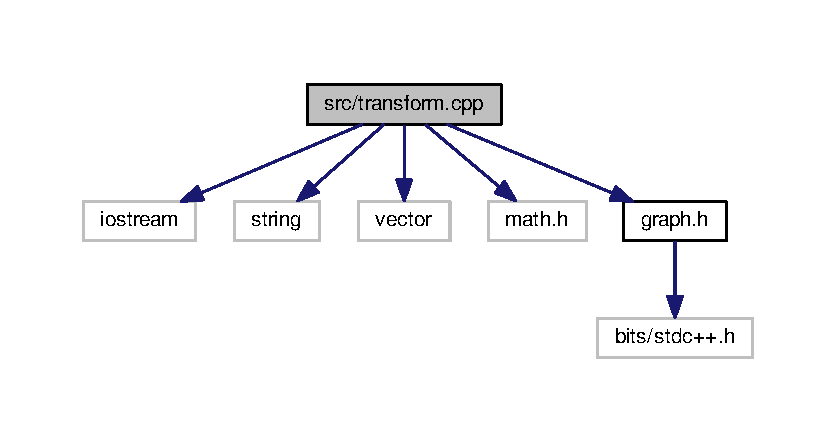
\includegraphics[width=350pt]{transform_8cpp__incl}
\end{center}
\end{figure}
\subsection*{Classes}
\begin{DoxyCompactItemize}
\item 
class \hyperlink{classtrans}{trans}
\end{DoxyCompactItemize}

%--- End generated contents ---

% Index
\backmatter
\newpage
\phantomsection
\clearemptydoublepage
\addcontentsline{toc}{chapter}{Index}
\printindex

\end{document}
